\section{Ciecierzyca w sosie curry}
\bigskip
\small
\begin{minipage}{0.45\textwidth}
    \noindent \textbf{Czas:} 45 minut \\
    \textbf{Poziom trudności:} łatwy
\end{minipage}
\begin{minipage}{0.45\textwidth}
    \noindent \textbf{Ilość sprzątania:} minimalna\\
    \textbf{Wymagany mysi sprzęt:} -
\end{minipage}
\normalsize
\vspace{0.5cm}

\begin{multicols}{2}

\subsection*{Składniki}
\begin{itemize}
    \item 1 duża cebula
    \item 2 łyżeczki nasion gorczycy (albo graniastej musztardy francuskiej)
    \item 1 puszka mleka kokosowego (opcjonalnie dodatkowo: małe opakowanie śmietany 18\%)
    \item 1 puszka krojonych pomidorów
    \item 3 puszki ciecierzycy
    \item 2 łyżki sosu sojowego
    \item 1-2 łyżeczki cukru trzcinowego (lub zwykłego)
    \item przyprawy
    \item olej do smażenia
    \item sól i pieprz do smaku
\end{itemize}

\columnbreak

\begin{figure}[H] \centering \fbox{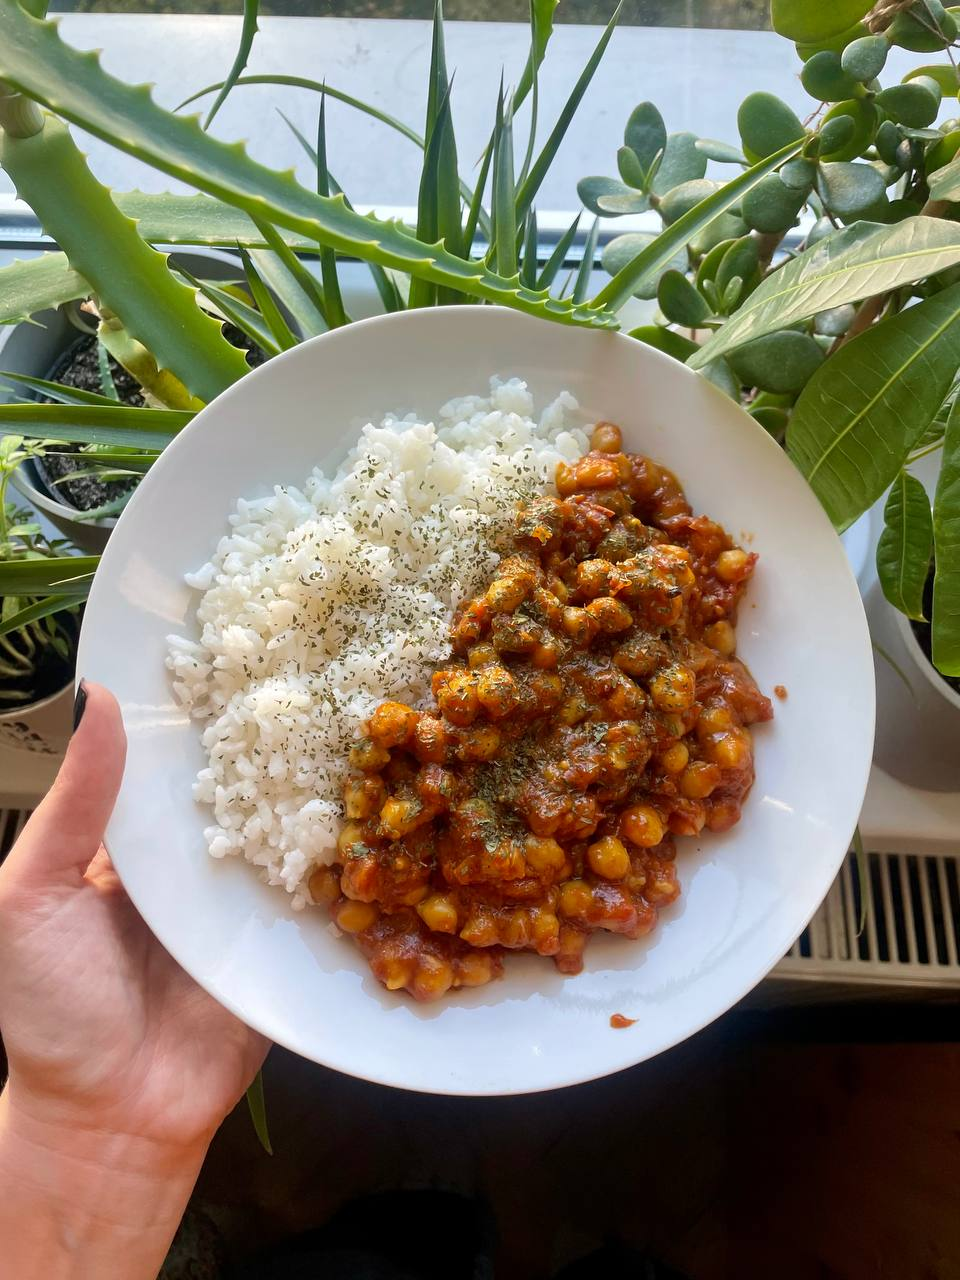
\includegraphics[width=0.35\textwidth]{images/curry.jpg}} \end{figure}

\end{multicols}

\vspace{0.5cm}

\subsection*{Instruktaż} \begin{enumerate} \item Cebulę posiekać na drobne kawałki i podsmażać do zeszklenia na oleju wraz z ziarnami gorczycy/musztardą i hojną szczyptą soli. \item Przez 30 sekund podsmażać przyprawy: po 3 łyżeczki kminu rzymskiego i curry, 2 łyżeczki kurkumy, chilli zgodnie z pożądanym poziomem ostrości (0.5-1 łyżeczka), hojna szczypta cynamonu. \item Wstrząsnąć puszkę z mlekiem kokosowym i wlać ją do garnka, dodać pomidory oraz sos sojowy i cukier. Dokładnie wymieszać i gotować aż zgęstnieje na średnim ogniu przez ok. 30 minut od momentu, gdy zacznie wrzeć, mieszając od czasu do czasu. \item Po upływie 30 minut dosolić do smaku, odsączyć ciecierzycę, wsypać do garnka i gotować na średnim ogniu ok. 15 minut, aż do uzyskania pożądanej konsystencji. \end{enumerate}

\vspace{0.5cm}

\small \subsection*{Propozycja podania} Ze świeżą kolendrą, z ryżem, z chlebkami indyjskimi naan z patelni.

\vspace{0.3cm}

\subsection*{Dodatkowe uwagi} Smakuje wybornie zarówno na zimno, jak i ciepło. Idealne do wzięcia w drogę lub do szkoły :)

\newpage
